\documentclass[linenumbers,RNAAS,trackchanges]{aastex631}
\usepackage[utf8]{inputenc}
\usepackage{hyperref}           % hrefs
\usepackage{natbib}             % for bibliography
\usepackage{float}              % figure positioning
\usepackage{svg}                % used for SVG images
\usepackage{tikz}
\usepackage{graphicx}           % used for non-SVG images
\usepackage{amsmath}  

% Search Query Metadata
%\shorttitle{title}

% Hyperlink setup
\hypersetup{
colorlinks=true,
linkcolor=blue,
urlcolor=blue
}

\tikzset{
  mynode/.style={fill,circle,inner sep=2pt,outer sep=0pt}
}

\begin{document}
\title{The Restricted Three Body Problem in Celestial Mechanics}
% [] is for ORCiD
\correspondingauthor{Ryan Charette, Abigail Iovino, Nicholas Davila}
\email{ryanacharette@gmail.com, abigail.iovino@gmail.com, ndavila@utexas.edu}
\author[0000-0000-0000-0000]{Ryan Charette}
\author[0000-0000-0000-0000]{Abigail Iovino}
\author[0000-0000-0000-0000]{Nicholas Davila}
\affiliation{The University of Texas at Austin College of Natural Science}




% 250 word limit for abstract
\begin{abstract}
In this paper, we derive the points of equilibrium (called Lagrange points) in a restricted three-body system containing Jupiter and the Sun. We use the Newton-Raphson method to numerically derive $L_1$, $L_2$, and $L_3$, since they are found at the roots shared between two (derived) equations of motion. The approach of our root-finding algorithm is to first make an initial guess for the roots based on the graph of the function (included), and then, by iterative process, to obtain a sufficiently precise result. For those points not located on the $x$-axis, namely $L_4$ and $L_5$, we use the fact they each form an equilateral triangle with the Sun and Jupiter to derive their location. 
\end{abstract}



% Use astrothesaurus numbers in place of num
% \keywords{keyword 1 (num) --- keyword 2 (num) --- keyword 3 (num)}
\keywords{Lagrange points (1) --- Lagrange mechanics (2) --- Lagrange point derivations (3) --- Sun-Jupiter Model (4) --- Restricted three-body system (5) --- Newton-Raphson method (6)s}
\section{\textbf{Introduction}} \label{sec:intro}
%in your introduction you will research the historical background of this topic and write a summary of the importance of this computation in celestial mechanics. We want references to papers in published journals not blogs on the internet

A restricted three-body problem occurs when three objects of ‘restricted size’ mutually interact with each other according to the Newtonian universal law of gravitation. In particular, the two large bodies move in a circular or elliptical orbit (the latter has been less studied) around their respective centers of mass, interacting with a third, much smaller body, which, owing to its small mass, has a negligible effect on their motion \cite[2]{Musielak_Quarles_2015}. A classic example of a restricted three-body system is the circular orbit of the Sun and the planets (large bodies) and asteroids and satellites such as moons (small bodies). The Earth–Moon–Sun system is one such example. 

The problem so to speak is that of describing the motion of the third body in this dynamic system. It was raised two centuries years ago by Euler in his lunar theories \cite[7]{szebehely2012theory}. Euler solved the problem involving two fixed bodies that interact with a third body via gravitational attraction \cite[5]{szebehely2012theory}. His solution, though useful in other fields, cannot be applied to celestial \cite[5]{szebehely2012theory}. Fifty years later, German mathematician Carl Gustav Jacob Jacobi discovered an integral of motion (known as the Jacobi Integral or Jacobi constant) that paved that way for future work. In the late nineteenth century, Poincaré published \textit{Les Méthodes Nouvelles de la Mécanique Célest} (New Methods of Celestial Mechanics), a three-volume work where he shed light on the unpredictability of the motions of the three bodies---the reason behind the problem's extreme difficulty---laying down the groundwork for chaos theory, changing the nature of modern approaches to the problem (see his approaches to differential equations), and earning him first place in a research competition in celestial mechanics organized by King Oscar II of Sweden and Norway \cite[2-4]{Musielak_Quarles_2015}. Today, the restricted three-body problem continues to fascinate mathematicians, astronomers, and physicists alike. The scientists and contributions mentioned cover hardly a sliver of the work in this field. The problem was and is motivation for developments in the field of numerical methods \cite[139]{hawking}.

\subsection{\textbf{Lagrange Points}} 
We know that objects move according to gravitational pull. In particular, a small object located at a point between two objects will be stationary if the gravitational pull of one large object exactly compensates for the gravitational pull of the other large object. There is one such point in a system of two fixed bodies. There are five such points in a system of three orbiting bodies (denoted $L_1$, $L_2$, $L_3$, $L_4$, and $L_5$). Points of this kind, unto which the two large bodies exert the same gravitational pull, are points of equilibrium. Euler discovered $L_1$, $L_2$, and $L_3$, and Joseph-Louis Lagrange (born Giuseppe Luigi Lagrancia in Turin, Italy) discovered $L_4$ and $L_5$. All five points are named “Lagrange points” after the latter mathematician and astronomer.  Those points discovered by Lagrange are considered ‘truly’ stable because gentle pulls (gravitational perturbations) are not enough to throw objects located at those points out of orbit (the Coriolis force curves the object’s path) so long as the ratio between the larger masses and smaller mass is sufficiently large. Thus, objects around these points are not inert. Because of their peculiar orbiting behavior, the stable area around $L_4$ and $L_5$ is significantly large and tends to accumulate space matter. Both $L_4$ and $L_5$ form an equilateral triangle with the two large bodies and are thus found at a 60-degree angle, but stable orbiting objects (called Trojans) have been found farther than 5 degrees from them  \cite[9]{Greenspan_2014}. Lagrange argued for the existence of such points using mathematics in 1772, but it was not until 1906 that astronomers, by discovering such Trojans, found astronomical evidence that he was correct \cite{Garner_2021}\cite[3]{Musielak_Quarles_2015}.

    \begin{figure}[H]
         \centering
         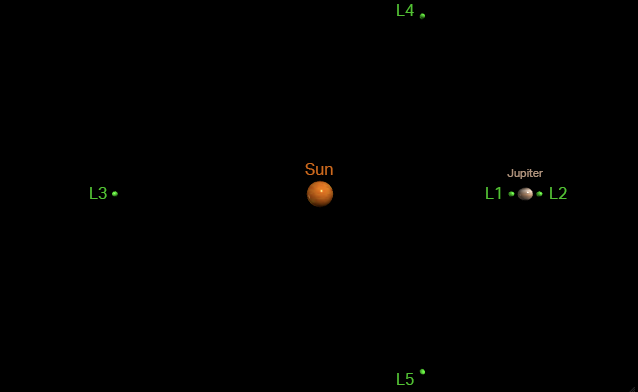
\includegraphics[width=0.6\textwidth]{Lagrange points model PS.png}
         \caption{3D (not to scale) model of the Lagrange points for a Sun-Jupiter system created using VPython. The locations of the Lagrange points on this model are the ones we obtained from our results in Table 1.}
    \end{figure}
\subsection{\textbf{Formal Problem Statement}}
In this paper we will be solving for the 5 Lagrange points in the Jupiter-Sun system to demonstrate the numerical methods used to simulate 2-body systems. For simplicity, we will work under the assumption that Jupiter's orbit is a circle with a radius of 5.2 AU. In order to solve for these points, we can create vector field of the gravitational forces in the Jupiter-Sun system and locate the points where the vectors cancel out to 0. An object at any such point will not be subject to any force and will therefore have an acceleration of 0 relative to Jupiter. The Lagrange points of Jupiter are of particular interest because at the stable points L4 and L5 are clusters of asteroids called the Trojan Asteroids. Astronomers believe these asteroids to be remains of the primordial material that formed the outer planets, and their study may reveal new information about the formation of the solar system \cite{Garner_2021}.

\vspace{1cm}
\section{\textbf{Equations and Numerical Methods}}
% You will state (or derive) the equations of motion that you will be solving and discuss the numerical method(s) that you chose to solve the problem.

Let $M_{1}$ and $M_{2}$  be the two masses with $M_{1} >> M_{2}$, and let $\vec{r_1}$ and $\vec{r_2}$ be their respective positions. Then using Newton's Law of Gravitation, $F=\frac{Gm_1 m_2}{r^2}$, then Kepler's Third Law, $P^2=a^3$ tells us that the total force exerted on a third, sufficiently small, mass $m$, at position $\vec{r}$ will be
$$\vec{F}=-\frac{GM_1 m}{|\vec{r}-\vec{r_1 } |^3}  (\vec{r }-\vec{r_1})-\frac{GM_2 m}{|\vec{r}-\vec{r_2 } |^3}  (\vec{r }-\vec{r_2})$$
Then by Newton's second law, the acceleration of the third mass can be described 
$$\vec{a}=-\frac{GM_1}{|\vec{r}-\vec{r_1}|^3}  (\vec{r}-\vec{r_1})-\frac{GM_2}{|\vec{r}-\vec{r_2}|^3}(\vec{r}-\vec{r_2})$$
The Law of Conservation of Angular Momentum suggests that objects in orbit around the Sun are contained on a single plane, so we can assume that there is no acceleration on the z-axis. Then if the Sun is positioned at $x=-R_\odot$ and Jupiter at $x=R_J$, the acceleration vector can be represented for an object located at $(x,y)$ by the equations
\[a_x (x,y)=-\frac{GM_\odot}{(x+R_\odot)^2+y^2 )^{3/2}}  (x+R_\odot)-
\frac{GM_J}{((x-R_J )^2+y^2 )^(3/2)}(x-R_J )\]
\[a_y (x,y)=-\frac{GM_\odot}{(x+R_\odot)^2+y^2 )^{3/2}}(y)-\frac{GM_J}{((x-R_J )^2+y^2 )^{3/2}} (y)\]
For an object to have rotate synchronously with Jupiter, it would need an acceleration such that $a(x,y)=[-\omega^2 x,-\omega^2 y$]  where $\omega$ is the angular velocity of Jupiter.Then combining with the equations above, we get that the Lagrange points are found when 
$$a_x (x,y)+\omega^2 x=a_y (x,y)+\omega^2 y=0$$
We can use Newton's Method, $x_{n+1}=\frac{x_n-f(x_n)}{f'(x_n)}$  to approximate the shared roots of $a_x (x,y)+\omega^2 x$ and $a_y (x,y)+\omega^2 y$. This will involve graphing the functions to find reasonable initial guesses for the roots and using an algorithm to improve our guess until a sufficiently precise value is reached. For computational efficiency, we will use a quasi- Newton method called Broyden's method, where the derivative is replaced with a Jacobian matrix. However, additional Lagrange points can be found that are not on the x-axis. For these points, we can construct a triangle between $M_{1}$, $M_{2}$, and $m$. 
$$\frac{GM_{1}(r-r_{1})}{|r-r_{1}|^3}+\frac{GM_{2}(r-r_{2})}{|r-r_{2}|^3}=\omega^2r=\frac{G(M_{1}+M_{2})}{|r_{1}-r_{2}|^3}$$
$$\alpha(r-r_{1})+\beta(r-r_{2})=r$$
$$\alpha r_{1} + \beta r_{2}=(\alpha + \beta -1)r$$ The above equation describes a line which is parallel to $r$. Since $r_{1}$ and $r_{2}$ are on the same line, then $m$ is either on the line connecting those two points, as solved for above, or $\alpha r_{1} + \beta r_{2}=0$. But $M_{1}r_{1} + M_{2}r_{2}=0$ and therefore $\frac{\alpha}{\beta}=\frac{M_{1}}{M_{2}}$. If $|r-r{1}|=|r-r_{2}|$ then let $S=|r-r{1}|=|r-r_{2}|$.
$\frac{M_1}{S^3}(r-r_{1})+\frac{M_2}{{S^3}}(r-r_{2})=\frac{(M_{1}+M_{2})r}{|r_{1}-r_{2}|^3}=S$
Therefore, the triangle constructed from points $M_{1}$, $M_{2}$, and $m$ is equilateral. We can use simple trigonometry to determine the location of the two remaining Lagrange points.
%%%%%%%%%%%%%%%%%%%%%%%%%%%%%%%%%%%%%%%%%%%%%%%%%%%%%%%%%%%%%%%%%%%%%%%%%%%%%%%%%%%%%%%%%%%

    \subsection{\textbf{Finding the First Three Lagrange Points}}
    
    In our model, which can be seen in Figure 1, the Sun is at the origin, and Jupiter is directly horizontal from the Sun at 5.2 AU (or about 7.779e11 m) away in the positive $\hat{x}$ direction with the Sun at the origin. Because of this, we can simplify our equations of motion by substituting y = 0. For the first three Lagrange points we were able to use the Newton-Raphson method for linear equations. \\
    
    \noindent
    We can find the first three $L_{\textup{points}}$ by making an intelligent guess for our Newton-Raphson method. The best place to look is along the x-axis where y = 0. So, if we plug in y = 0 to our equations of motion we get:
    
    \begin{equation}
    \ 0 = - \frac{G M_{\bigodot} (x + R_{\bigodot})}  {((x + R_{\bigodot})^2 + [0])^{3/2}}
    \ - \frac{G M_j (x - R_j)} {((x - R_{j})^2 + [0])^{3/2}}
    \ + \omega^2 x
    \label{eq: omega_x_0_pre} \tag{1}
    \end{equation}
    
    \begin{equation}
    \ 0 = - \frac{G M_{\bigodot} [0]}  {((x + R_{\bigodot})^2 + [0])^{3/2}}
    \ - \frac{G M_j [0]} {((x - R_{j})^2 + [0])^{3/2}}
    \ + \omega^2 [0]
    \label{eq: omega_y_0_pre} \tag{2}
    \end{equation}
    
    \noindent
    Equation $\eqref{eq: omega_y_0_pre}$ becomes 0 when we plug in 0, and equation $\eqref{eq: omega_x_0_pre}$ becomes a simplified version:

    \begin{equation}
    \ 0 = - \frac{G M_{\bigodot}}{(x + R_{\bigodot})^2}
    \ - \frac{G M_j} {(x - R_{j})^2}
    \ + \omega^2 x
    \label{eq: omega_x_0_y0} \tag{3}
    \end{equation}
    
    \noindent
    Where G is the gravitational constant 6.67408e-11 $m^3/kg * s^2$, $M_{\bigodot}$ is the mass of the Sun 1.9891e30 kg, $M_j$ is the mass of Jupiter 1.8981e27 kg, $\omega$ is the angular velocity 1.6799e-8 rad/s, $R_{\bigodot}$ is the distance of the Sun from the center of mass and $R_j$ is the distance of Jupiter from the center of mass.\\

    \noindent
    To make smart guesses for the roots we first want to plot our equations of motion. Since for the first three $L_{\textup{points}}$ we only care about the motion or acceleration in x, but want to know where y equals 0, we plot our original equations of motion before plugging y for 0 (so we can visually inspect where y = 0). Figure 2 shows how we made our guesses, and Table 1 shows our results after inputting guesses into our Newton-Raphson method for $L_{\textup{points}}$ 1 through 3.

    \begin{figure}[H]
         \centering
         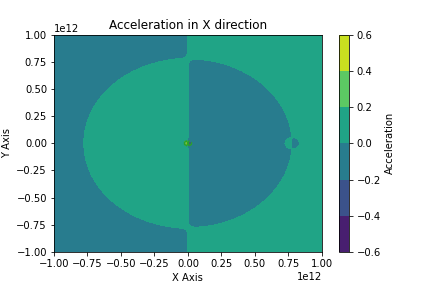
\includegraphics[width=0.6\textwidth]{ax_plot.png}
         \caption{ The plot of the equation $\displaystyle 0 = - \frac{G M_{\bigodot} (x + R_{\bigodot})}{((x + R_{\bigodot})^2 + y^2)^{3/2}} - \frac{G M_j (x - R_j)} {((x - R_{j})^2 + y^2)^{3/2}} + \omega^2 x$ The plot is from -10e11 m to 10e11 m for both x and y in the previous equation. We inspected the plot to find where dark green would change to light green and y equaled zero, and those regions were where we guessed.}
    \end{figure}
    
    \subsection{\textbf{Finding the Fourth and Fifth Lagrange Points}}
    
    \begin{figure}[H]
         \centering
         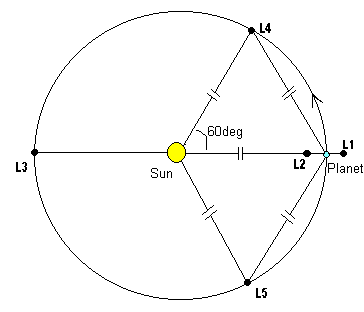
\includegraphics[width=0.4\textwidth]{lpoints.png}
         \caption{Drawing of the five Lagrange points for two massive bodies rotating about their center of mass. For this subsection, we are focused on L4 and L5 which form the vertices of an equilateral triangle with the main two masses of the system. The logic and derivation of this can be found in the \textbf{EQUATIONS AND NUMERICAL METHODS}. Image source: \url{https://www.spaceacademy.net.au/library/notes/lagrangp.htm}}
    \end{figure}
    
    Using the logic and derivations from the \textbf{EQUATIONS AND NUMERICAL METHODS} section, Figure 3, and the derivations from the Neil J. Cornish (PDF on the class Canvas), we have two equations to calculate L4 and L5. Those equations are:
    \begin{equation}
        L4: \left(\frac{R}{2} \left(\frac{M_1 - M_2}{M_1 + M_2} \right), \frac{\sqrt{3}}{2}   \right)
        \label{eq: L4} \tag{4}
    \end{equation}
    
    \begin{equation}
        L5: \left(\frac{R}{2} \left(\frac{M_1 - M_2}{M_1 + M_2} \right), -\frac{\sqrt{3}}{2} R  \right)
        \label{eq: L5} \tag{5},
    \end{equation}
    
    \noindent
    where R is the distance from the Sun ($M_1$) to Jupiter ($M_2$) in meters. Now we just need to plug in our values and get our results.
    
    

%%%%%%%%%%%%%%%%%%%%%%%%%%%%%%%%%%%%%%%%%%%%%%%%%%%%%%%%%%%%%%%%%%%%%%%%%%%%%%%%%%%%%%%%%%%

\section{\textbf{Results}}
%You will explain and interpret your results. Discuss the stability of these points.
\begin{table}[H]
    \centering
    \begin{tabular}{|c|c|c|}
         \hline
         $L_{\textup{point}}$ &  Location in x,y (meters) & Stability \\
         \hline
         $L_1$ & (7.25684e11, 0) & Unstable \\
         \hline
         $L_2$ & (8.31758e11, 0) & Unstable \\
         \hline
         $L_3$ & (-7.77294e11, 0) & Unstable \\
         \hline
         $L_4$ & (3.882084e11, 6.736812e11) & Stable \\
         \hline
         $L_5$ & (3.882084e11, -6.736812e11) & Stable \\
         \hline
    \end{tabular}
    \caption{Our results for calculating the Lagrange points. Points $L_1$, $L_2$, and $L_3$ were found using a Newton-Raphson method. Points $L_4$ and $L_5$ were found using an equilateral triangle method.}
    \label{tab:data_tab}
\end{table}
Given the mathematical assumptions of our model, these results are as expected; $L_1$ and $L_2$ are equidistant from Jupiter, and the distance between the Sun and $L_3$ is equal to the distance between the Sun and Jupiter. Additionally, $L_4$ and $L_5$ form equilateral triangles with the Sun and Jupiter. Of these 5 points, only $L_4$ and $L_5$ are considered stable (i.e. resistant to gravitational perturbations) and $L_1$, $L_2$, and $L_3$ are unstable so long as 
\[\frac{M_1}{M_2} \geq \frac{25 + 3\sqrt{60}}{2} =24.9599. \] Proof of this fact can be found in a Thomas Greenspan's paper \textit{Stability of the Lagrange Points, $L_4$ and $L_5$}\cite[6-8]{Greenspan_2014} It is critical to consider stability of Lagrange points when engaging with real-world applications, since objects will rarely be found an exact point, but near it.

\section{\textbf{Conclusion}} \label{sec:summary}
%you will conclude by reflecting on how well you solved the problem. You will discuss any future work that you could have done by adding the gravitational effects of the moons of Jupiter and other planets like Saturn on the Lagrangian points. 

Our model makes several assumptions for mathematical simplicity that will cause our simulation to differ from reality. Most significantly is our assumption that Jupiter's orbit around the Sun is circular. Kepler's First Law tells us that orbits are elliptical with one of the foci being located at the Sun. Jupiter has an orbital eccentricity of 0.0487, indicating a roughly circular orbit (source below). As such, this assumption introduces an average error of 4.87\%  when Jupiter is not exactly 5.2 AU away from the Sun. 

Further error is caused by standard assumptions of Newtonian physics, primarily that the Sun is stationary, Jupiter is point-like, that both bodies are perfectly spherical, non-rotating, and uncharged, and that no energy is lost in the Jupiter-Sun system through mechanisms such as gravitational radiation. These assumptions are standard and result in negligible error.

A more accurate model could be constructed by accounting for the impact of nearby massive objects on the positions of the Lagrange points. The Galilean moons are likely to have a noticeable effect on the $L_1$ and $L_2$ points in particular, given their relatively short distance from Jupiter. The other Lagrange points may be more significantly affected by the gravitational influence of Saturn. 

With these factors in mind, we estimate that our model is reasonably accurate, with a margin of error of $\sim\pm5\%$. 

%source on eccentricity of Jupiter's orbit (https://nssdc.gsfc.nasa.gov/planetary/factsheet/jupiterfact.html)

\section{\textbf{Acknowledgment}} \label{sec:acknowledgment}
Ryan, Abi, and Nick would like to thank Brett for his timely manner and thoroughness when answering all of our questions, even in non-working hours. We would also like to thank Professor Mitra for his guidance and support, and all of our classmates for their shared wisdom. 

\newpage
\bibliographystyle{aasjournal}
\bibliography{bibliography.bib}

\end{document}
